\section{Organisation du groupe}
\subsection{Présentation du groupe}
\paragraph{Alexandre de Lingua de Saint Blanquat :}
Étudiant à l'UPSSITECH, j'ai passé mon baccalauréat au Cambodge avant de faire un IUT GEII. J'ai été accepté à l'UPSSITECH en Système Robotique et Interactif (SRI). J'ai été le chef de projet et j'ai contribué à toutes les parties. J'ai fait la page WEB, la gestion du Git et du GitHub, les tests pour le chronomètre et le programme principal. J'ai aussi proposé au groupe les différents composants et assemblé le prototype. J'étais la personne sur qui les membres du groupe pouvaient compter quand ils étaient en difficultés.

\paragraph{Mohamed EL MOURABIT:}
Étudiant en M1 Système Robotique et Interactifs, je suis issue d'une formation en GEII (Génie électrique et informatique industrielle). J’ai ensuite intégré l’UPSSITECH en L3 en SRI (Système Robotique et Interactifs). Sur ce projet , j'ai principalement travaillé sur la partie programmation. 

\paragraph{Hugo DIRINGER :}
Etudiant en M1 Système Robotique et Interactifs, j’ai débuté pour un DUT GEII (Génie électrique et informatique industrielle). J’ai continué mes étude en intégrant le cursus SRI (Système Robotique et Interactifs) de l’UPSSITECH. Durant ce projet, j’ai eu à m'occuper de plusieurs taches incluant la création et l'utilisation du réseau, l'intégration des différentes partie du projet et la modélisation des boîtier.

\paragraph{Hippolyte Catteau :}
Étudiant en M1 Système Robotique et Interactifs, j'ai d'abord étudié pour obtenir mon DUT GEII (Génie électrique et informatique industrielle). J’ai ensuite intégré l’UPSSITECH en L3 en SRI (Système Robotique et Interactifs). Durant le projet, j'ai été la personne qui était toujours en contact avec le client et qui s'occuper de gérer les différents rendez-vous avec ce dernier. J'ai aidé sur la partie programmation et j'ai réaliser le cahier des charges et le manuel d'utilisation du produit.

\paragraph{François Mahé :}
Étudiant en M1 Système Robotique et Interactifs, j’ai commencé ma formation par une license en Sciences Fondamentales Appliquées suivant une orientation vers l’informatique. J’ai par la suite intégré le cursus de l’UPSSITECH en L3. Durant ce projet j’ai principalement travaillé sur le prototypage du boîtier et l’étude des solutions déjà existantes.

\subsection{Outils utilisés}
Durant la durée du projet nous avons utilisés plusieurs outils :

\paragraph{Outils de gestion de projet :}
\begin{itemize}
    \item Messenger : Communication interne du groupe
    \item Git : gestion du code
    \item GitHub : gestion des différentes tâches du groupes
\end{itemize}

\begin{center}
  \makebox[\textwidth]{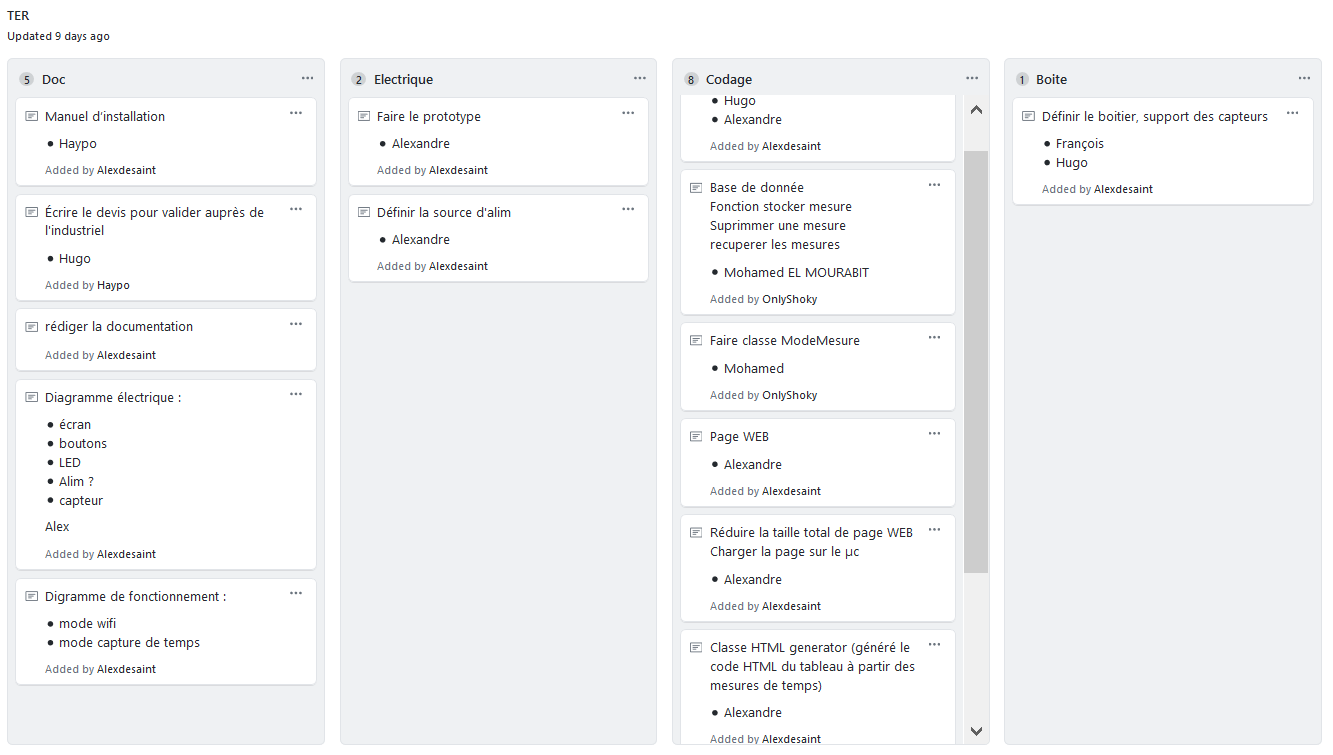
\includegraphics[width=13cm]{photoHippo/gestionDeProjetTER}}
  
  Diagramme d'organisation du groupe sur le GitHub
\end{center}

\paragraph{Outils techniques :}
\begin{itemize}
    \item Visual Studio Code : Editeur de texte
    \item Platform IO : Compiler le projet et le téléverser
    \item OpenSCAD et Auto Desk Fusion 360 pour la modélisation 3D des boitiers
    \item Adobe After Effects pour le montage de la vidéo
\end{itemize}
